% version 1.00, date 05/11/16, auteur Kafui Atanley
% version 2.00, date 28/11/16, auteur François Decq
\subsection{Fonctionnalité 9}

La fonctionnalité 9 consistera à planifier les interventions de type frimousse c'est-à-dire qu'un intervenant s'attribue une intervention de type frimousse.
Lors de chaque affectation, un e-mail d'information de prise en charge de la demande par l'équipe d'intervenants sera envoyé à l'établissement demandeur ainsi qu'au responsable de l'activité frimousse.
La figure \ref{courrielPrisChargeFrimousse} présente la maquette de cet email d'information de prise en charge. 
Une intervention ne peut être attribuée qu'à un utilisateur.
  La figure \ref{visualiserESTAttribuer} présente le diagramme de cas d'utilisation sur la visualisation et l'attribution des interventions.\\

\begin{figure}[H]
	\centering
	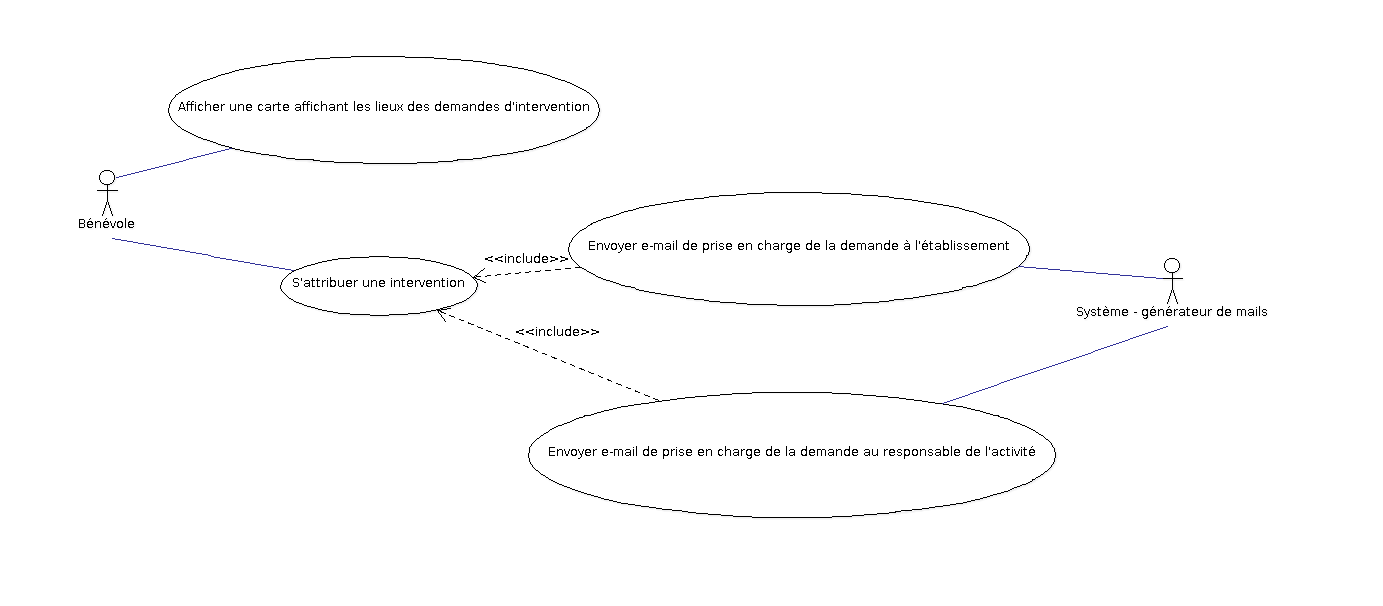
\includegraphics[scale=0.4]{images/casDUtilisation/fonctionnalite5Attribution.png}
	 \caption{Cas d'utilisation~: Visualiser les demandes et s'attribuer des interventions}
	 \label{visualiserESTAttribuer}
\end{figure}

% Figure : version 1.00, date 24/02/16, auteur Michel Cressant
\begin{figure}[H]
	\centering
	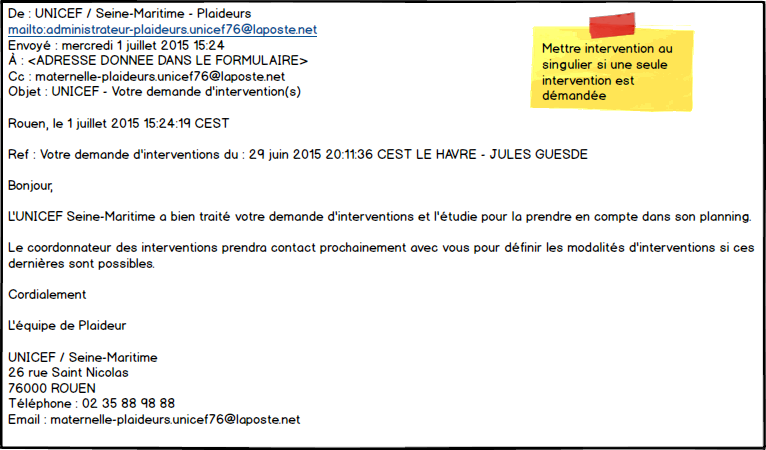
\includegraphics[scale=0.675]{images/maquettes/fonctionnalite5MailDePriseEnCharge.png}
	\caption{Maquette~: Email de prise en charge d'une intervention}
	\label{courrielPrisChargeFrimousse}
\end{figure}
